\documentclass{ltjsbook}
\usepackage{docmute} 
\usepackage{../../myStyle} 

\begin{document}
% \chapter{多次元尺度構成法}
\chapter{Multidimensional Scaling Method}
\label{x15_MDS}
% 今回は\keyterm{多次元尺度構成法}{たじげんしゃくどこうせいほう}{Multi-Dimensional Sacling; MDS}について解説します。
This time, I will explain about the Multi-Dimensional Scaling (MDS) method.
% ここまで分散共分散行列を分解するところから，クロス表のような\keyterm{名義尺度水準}{めいぎしゃくどすいじゅん}のデータを分解するところまでやってきました。
We have come this far, from decomposing the variance-covariance matrix to decomposing data at the nominal scale level, such as contingency tables.

% 多次元尺度構成法は，分散共分散行列を扱う線形モデルよりはやや仮定が緩く，また数量化のように解析者が数字を与えることを目的にするというよりは，その名の通り尺度を作ろうとしているという意味で心理学的・心理測定的なモデルだといえるでしょう。
The multidimensional scaling method is a somewhat looser assumption than the linear model that deals with the variance-covariance matrix, and it can be said that it is a psychological/psychometric model in the sense that it aims to create scales rather than the analyst aiming to provide numbers like quantification.

% 私たちが単位もない不確かなものを対象にしながらもそれを測定するモノサシをつくることができるのは，2つの対象にたいしてその比較をして一方が他方よりも大である，ということが言えるからでしょう。
The reason we can create a ruler to measure something uncertain without units is probably because we can compare two things and say that one is larger than the other.
% 記号を使って言えば，$x$と$y$を比べて$x \succeq y$である，ということから，尺度上の値$p \ge q$を対応させるということが，尺度を作るということです\footnote{経済学では学問の最初の段階で，財を源とした集合に対する二項関係$x \circ y$を定義し，それを効用関数$u$で実数領域に写像して$u(x) \ge u(y)$を考える，といった基本的な原理を抑えます。心理学ではなぜか，「集合」「元」「二項関係」という基本的な比較の要素について考えることなく，その分析ツールだけがどんどんと発展してきています。}。
In terms of symbols, constructing a scale means corresponding a value on the scale where $p \ge q$ from the point that $x \succeq y$ when comparing $x$ and $y$\footnote{In economics, at the first stage of academic research, a binary relationship $x \circ y$ is defined for a set derived from goods, and it is imaged in the real number area by a utility function $u$, and $u(x) \ge u(y)$ is considered. It is a basic principle. Interestingly, in psychology, the basic elements of comparison such as "set", "element", "binary relationship" are not considered, and only its analytical tools have been evolving.}.
% このとき比較する2つが重さや広さのような物理的なものであればわかりやすいですし，「痛み」や「喜び」といった心理的な要素であっても構いません。あるいは「より賛成」といった態度表明のようなものでも良いかもしれません。
It is easy to understand if the two things being compared are physical things like weight or size, and it is also okay if they are psychological elements such as "pain" or "joy". Alternatively, it may be something like a statement of attitude, such as "more in favor".
% この比較から出てくる関係は，分散共分散や相関係数のように強い線形の過程を置かなくても，より緩やかに\keyterm{距離}{きょり}{distance}という考え方で表現されます\footnote{後述しますが，相関係数も距離の一種と考えられます。}。
The relationship that emerges from this comparison is represented more gently by the concept of \keyterm{distance}{きょり}{distance}, without the need for a strong linear process like variance covariance or correlation coefficients\footnote{As will be discussed later, the correlation coefficient can also be considered a type of distance.}.

% MDSは距離行列を固有値分解するモデルです。それではこの方法について内容を見ていきましょう。
MDS is a model that decomposes distance matrices into eigenvalues. Let's take a look at the contents of this method.

% \section{多次元尺度構成法}
\section{Method of Multidimensional Scaling}
% Rにはサンプルデータとして\texttt{eurodist}というヨーロッパ各地の都市間距離のデータが用意されています。表\ref{tbl::15_01}にその一部を示します。
There is a data set called \texttt{eurodist} in R that provides information on the distance between various cities in Europe. Part of it is shown in Table \ref{tbl::15_01}.

\begin{table}[ht]
    \centering
    \caption{ヨーロッパ都市間距離データの一部}
    \begin{tabular}{l|rrrrrr}
                  & Athens & Barcelona & Brussels & Calais & Cherbourg & Cologne \\
        \hline
        Athens    & 0      &           &          &        &           &         \\
        Barcelona & 3313   & 0         &          &        &           &         \\
        Brussels  & 2963   & 1318      & 0        &        &           &         \\
        Calais    & 3175   & 1326      & 204      & 0      &           &         \\
        Cherbourg & 3339   & 1294      & 583      & 460    & 0         &         \\
        Cologne   & 2762   & 1498      & 206      & 409    & 785       & 0       \\
        \hline
    \end{tabular}
    \label{tbl::15_01}
\end{table}


% 元のデータは$21 \times 21$のサイズです。表から，たとえばアテネ(Athens)とバルセロナ(Barcelona)の距離が3313km，と言うことが読み取れます。表の右上が空白になっていますが，これは\keytermL{距離行列}{きょりぎょうれつ}が\keytermL{対称行列}{たいしょうぎょうれつ}なので，ムダな情報を表示しないようにしているからです。アテネとバルセロナの距離は，バルセロナとアテネの距離に等しいですからね。
The original data is of size $21 \times 21$. From the table, we can read, for example, that the distance between Athens and Barcelona is 3313km. The top right part of the table is blank, because this is a distance matrix, which is a symmetrical matrix, so we avoid displaying redundant information. After all, the distance from Athens to Barcelona is equal to the distance from Barcelona to Athens.

% さて距離行列はこのように，\keytermL{正方行列}{せいほうぎょうれつ}ですから，\keytermL{固有値分解}{こゆうちぶんかい}をすることで\keytermL{基底}{きてい}を求めることができます。基底は座標を形成する基本単位ですから，それを使って各変数の位置にあたる座標を計算できます\footnote{厳密には距離行列$\bm{D}$そのものではなく，それを二重中心化した行列の固有値分解になりますが，本質的には変わりません。詳しくは\textcite{Okada19940115}などを参照のこと。}。このように距離行列から座標を求めて，変数をプロットすることで変数間関係を可視化する手法のことを\keyterm{多次元尺度構成法}{たじげんしゃくどこうせいほう}{Multi-Dimensional Scaling: MDS}と言います。
Now, the distance matrix is a \keytermL{square matrix}{せいほうぎょうれつ}, so you can find the \keytermL{basis}{きてい} by \keytermL{eigenvalue decomposition}{こゆうちぶんかい}. Since the basis forms the basic unit of the coordinates, you can calculate the coordinates corresponding to the position of each variable using it\footnote{Strictly speaking, it's not the distance matrix $\bm{D}$ itself, but the eigenvalue decomposition of the double centered matrix, although essentially it doesn't change. For more details, please refer to \textcite{Okada19940115} and the like.}. This method of finding the coordinates from the distance matrix and plotting the variables to visualize the relationship between the variables is called \keyterm{Multidimensional Scaling: MDS}{たじげんしゃくどこうせいほう}.

% 試しに\texttt{eurodist}データをMDSで2次元プロットしてみましょう。
Let's try to plot the \texttt{eurodist} data in 2D using MDS as a test.
% これを実行するコードは簡単で，\texttt{eurodist}データのようにデフォルトで組み込まれている\texttt{cmdscale}関数を使います。
The code to execute this is simple, and it uses the function \texttt{cmdscale} that is built-in by default like the \texttt{eurodist} data.

\begin{lstlisting}[language=C++,label={code:x15_01},caption={計量MDSの実践と描画}]
library(ggrepel)
# MDSを実行
result.MDS1 <- cmdscale(eurodist,k=3)
# y軸反転させつつ描画
g <- result.MDS1 %>%
  as.data.frame() %>%
  dplyr::mutate(label = rownames(.)) %>%
  ggplot(aes(x = V1, y = V2, label = label)) +
  geom_point() +
  geom_text_repel() +
  xlim(-2500, 2500) +
  ylim(2500, -2500) +
  xlab("dim 1") +
  ylab("dim2")
\end{lstlisting}


% \paragraph{コード解説}
\paragraph{Code Explanation}
\begin{description}
    \item[1行目] \verb|ggplot2|でラベルをプロットするときに，綺麗な配置にしてくれる\verb|ggrepel|パッケージを使います。このコードを実行するときに持っていない人は，インストールしておいてください。
    \item[3行目] \verb|cmdscale|関数に\verb|eurodist|データを与えています。\verb|k=3|は3次元解を出すように指定しています。地球は球体ですから，地球上の地理は3次元で表現できますよね。
    \item[5-14行目] \verb|ggplot2|による描画です。結果オブジェクトである\verb|result.MDS|をデータフレームにし，行の名前になっていた都市名を変数として格納したのち，散布図のようにプロットしています。
\end{description}


\begin{figure}[ht]
	\begin{center}
		\includegraphics[width=0.8\linewidth,keepaspectratio]{../images/15_MDS/Rplot15_01.png}
		\caption{MDSのプロット}
		\label{fig::15_01}
	\end{center}
\end{figure}


% 図\ref{fig::15_01}をみると，上の方にストックホルム(Stockholm)があって，右下にアテネが，中央にパリ(Paris)が・・・といった配置になっています。地球上の位置と完全に一致しているとは言えませんが，それでも概ねうまくプロットできていますね\footnote{完全に一致しない理由は，地球が球面であるのに対し平面にプロットしたから，と言うのもあります。}。このように，距離関係だけから地図を作ることができるというのが，MDSという手法なのです。
Looking at Figure \ref{fig::15_01}, you can see Stockholm at the top, Athens at the bottom right, and Paris in the center... and so on. It can't be said that it perfectly matches their positions on the globe, but overall, it is well plotted\footnote{ One reason it does not perfectly match is because we are plotting onto a flat surface from a spherical one.}. This method, called MDS, allows us to create a map from just the distance relationships.


% \section{距離と心理学のデータ}
\section{Data on Distance and Psychology}
\label{distance}
% MDSは距離関係だけから地図を作る方法でした。因子分析は相関関係から次元を作る方法でした。この2つの手法はとても似ています。というのも，相関関係と言うのが変数と変数の近さ・遠さ，つまり距離を表しているとも言えるからです。
MDS is a method of creating maps from distance relationships alone. Factor analysis is a method of creating dimensions from correlation relationships. These two methods are very similar. This is because a correlation relationship can also be said to express the nearness or distance between variables, in other words, the distance.
% あらためて\keyterm{距離}{きょり}{distance}とは何かを考えてみましょう。2点$x,y$の距離を$d(x,y)$とすると，距離とよばれる数字の条件は次のようになります。
Let's reconsider what \keyterm{distance} is. If we denote the distance between two points $x, y$ as $d(x, y)$, the numbers called distance are determined by the following conditions.
\begin{description}
	\item[非負性] $d(x,y)\ge 0$
	\item[非退化性] $d(x,y)=0 \Leftrightarrow x=y$
	\item[対称性] $d(x,y)=d(y,x)$
	\item[三角不等式] $d(x,z) + d(z,y) \ge d(x,y)$
\end{description}

% もっとも一般的に使われるのはユークリッド距離で，2次元座標$(x_1,y_1),(x_2,y_2)$があった時のユークリッド距離は次のように計算します。
The most commonly used is the Euclidean distance. When there are two-dimensional coordinates $(x_1,y_1),(x_2,y_2)$, the Euclidean distance is calculated as follows.
\[ \sqrt{(x_1-x_2)^2+(y_1-y_2)^2} \]
3次元座標$(x_1,y_1,z_1),(x_2,y_2,z_2)$の場合は項を増やすだけです。
\[ \sqrt{(x_1-x_2)^2+(y_1-y_2)^2+(z_1-z_2)^2} \]
% このようにして計算される距離ですが，上の条件を考えると何も二乗してルートを取らなくても絶対値を足し合わせるような方法でも構いません。たとえば2次元座標の場合は，次のような計算でもいいのです。
The distance calculated in this way may be simply summed up by absolute values without squaring or taking the root, considering the above conditions. For example, in the case of two-dimensional coordinates, the following calculations would be acceptable.
\[ |x_1-x_2|+|y_1-y_2| \]
現にこのような距離のことを\keyterm{マンハッタン距離}{まんはったんきょり}{Manhattan distance}といいます。二乗ではなくn乗してn乗根をとる，という形で一般化することもできます。
\[ d(x,y) = \left( \sum_{i=1}^n |x_i - x_j|^p\right)^{\frac{1}{p}} \]
% これは\keyterm{ミンコフスキー距離}{みんこふすきーきょり}{Minkowski distance}という名前がついています。他にもマキシマム距離，バイナリ距離，チェビシェフの距離，キャンベラ距離などがあり，いずれもRの\texttt{dist}関数のオプションで選ぶことができますので，ヘルプなどを参照してみてください。
This is called the Minkowski distance. There are also other distances such as the maximum distance, binary distance, Chebyshev distance, Canberra distance, and others, all of which can be selected as options in R's dist function. Please refer to the help and other resources for more information.

% また，相関係数$r_{ij}$は$-1 \le r_{ij} \le +1$の範囲にありますが，この絶対値から$1-|r_{ij}|$とするとこれも距離の条件に当てはまります。どの程度類似しているかというのも，距離と考えることができるのです。
Also, the correlation coefficient $r_{ij}$ falls within the range of $-1 \le r_{ij} \le +1$, but if we take the absolute value as $1-|r_{ij}|$, this also fits the condition of distance. The extent to which they are similar can also be considered a distance.

% ここまでは数学的な距離のバリエーションでしたが，次に心理学的な意味に目を向けてみましょう。
So far we have discussed variations in mathematical distance, but let's turn our attention to psychological meanings next.
% 距離とは類似度でもありますから，何を距離と見なすかによって，さまざまな心理学的刺激がデータを形作ることになります。
Distance is also a similarity, so depending on what you consider as distance, various psychological stimuli will shape the data.

% たとえば評定尺度で，n個の項目で何らかの評価をしてもらったとします。$x_{ij}$を$i$番目の項目における対象$j$の評定値だとすると，
For example, consider a rating scale in which an evaluation is made on n items. Let $x_{ij}$ be the rating value of target $j$ on the $i$th item.
% $d(j,k) = \sqrt{\sum_{i=1}^N (x_{ij}-x_{ik})^2 }$とすれば対象の類似度が計算できます。
If you define $d(j,k) = \sqrt{\sum_{i=1}^N (x_{ij}-x_{ik})^2 }$, you can calculate the similarity of the target.
% ほかにも何らかの刺激A,Bについて，AかBかの判断をさせた時に混同してしまった混同率や，単語と単語の連想価，刺激の汎化勾配，反応潜時，ソシオメトリックなデータなど，いろいろなものが「類似しているかどうか」の指標として使えます\footnote{これらデータの例に関しては\textcite{Takane198002}のPp.14--27を参照してください。}。尺度評定よりも，具体的な2つの刺激が似ているかどうかの反応の方がやりやすい，というのは誰しも実感としてわかることではないかと思います。
When making a judgment on some stimuli A or B, various things such as the confusion rate at which they got confused, the associative value of words, the generalization gradient of stimuli, reaction latency, sociometric data, etc., can be used as indicators of whether they are "similar or not"\footnote{For examples of these data, please refer to Pp.14-27 of \textcite{Takane198002}.}. I think everyone can intuitively understand that it's easier to respond to whether two specific stimuli are similar or not, rather than making a scale evaluation.

% 類似度のデータが得られれば，それを距離と見做してMDSにかければ，変数間の関係を地図に描くことができるわけです。このように応用可能な領域が非常に広いことも，MDSの利点であると言えるでしょう。
If similarity data can be obtained, by treating it as a distance and applying it to MDS, we can map the relationship between variables. The fact that it can be applied to a very wide range of fields can also be said to be an advantage of MDS.

% \section{非計量多次元尺度法}
\section{Nonmetric Multidimensional Scaling Method}

% さて心理学的なさまざまな刺激が，MDSによって可視化できるということがわかってきました。距離行列が構成できれば，後の分析は何とでもできるわけです。
Now we understand that various psychological stimuli can be visualized through MDS. If a distance matrix can be constructed, it is possible to carry out any subsequent analysis.
% ただし，この場合の距離行列とは，間隔尺度水準以上であることが必要です。
However, in this case, the distance matrix must be at an interval scale level or higher.
% しかし心理学的な刺激に対する反応をデータ化する時は，同時に被験者はそこまで鋭敏に反応しているのか，いいかえれば本当に間隔尺度水準以上の精度で判断できているのかな，という人間側の問題が気になりますね。そこまで人間は鋭敏無反応をしていないかもしれません。
When quantifying the response to psychological stimuli, at the same time, we may wonder whether the subject is responding that sensitively, or in other words, whether they can really judge with more than interval scale-level precision. We might worry about this human issue. Humans may not be reacting that sensitively.

% でも大丈夫。MDSは仮定を緩めたモデルがあります。\keyterm{非計量的多次元尺度構成法}{ひけいりょうてきたじげんしゃくどこうせいほう}{Non-Metric Multi-Dimensional Scaling}と呼ばれる手法がそれです。非計量MDSでは，対象$j$と$k$の類似度を$\delta_{jk}$とし，分析によって埋め込む多次元空間での距離を$d_{jk}$とすると，
But it's okay. There is a model that relaxes the assumptions of MDS. This method is called Non-Metric Multi-Dimensional Scaling. In non-metric MDS, the similarity between object $j$ and $k$ is denoted as $\delta_{jk}$, and the distance in the multi-dimensional space embedded by the analysis is denoted as $d_{jk}$.

% $$ \delta_{jk} > \delta_{lm} \mbox{ならば}d_{jk}\le d_{lm} $$
"If δjk > δlm, then djk ≤ dlm"

% のように，イコールではなく順序関係だけ保持して座標を求めます。この手法では，元データが順序尺度水準程度の情報しか持っていなくても地図を描くことができるのです。人間の判断はせいぜいが順序尺度ぐらいですから，「より類似している($\delta_{jk} > \delta_{lm}$)」のであれば「より近くにある($d_{jk}\le d_{lm} $)」というぐらいの配置の方が良いかもしれません。
As such, it maintains only the order relationship, not equality, to determine the coordinates. With this method, it's possible to draw a map even if the original data only contains information at the ordinal scale level. Since human judgment is at best a ordinal scale, if "more similar ($\delta_{jk} > \delta_{lm}$)" then it might be better to have a layout that's "closer ($d_{jk}\le d_{lm}$)."


% 表\ref{tbl::15_01}に示したような物理的距離であれば，間隔尺度水準の情報であることは間違いありません。その場合には，最初に示した固有値分解による手法を使います。これは非計量MDSに対して，\keyterm{計量的多次元尺度構成法}{けいりょうてきたじげんしゃくどこうせいほう}{Metric Multi-Dimensional Scaling}と呼ばれています。
As shown in Table \ref{tbl::15_01}, there is no doubt that it is information at the interval scale level if it is a physical distance. In that case, use the method of eigenvalue decomposition shown first. This is called Metric Multi-Dimensional Scaling for non-metric MDS.


% \subsection{非計量多次元尺度法の例}
\subsection{Examples of Non-metric Multidimensional Scaling Method}

% 心理学ではデータの性質上，非計量MDSのほうが便利なことが多いでしょう。計量MDSでも非計量MDSでも，Rでは簡単な関数で実行できます。ここでは\verb|MASS|パッケージに含まれる\verb|isoMDS|関数を使って実践してみます。
In psychology, due to the nature of the data, non-metric MDS is often more convenient. Both metric and non-metric MDS can be executed with simple functions in R. Here, let's practice using the isoMDS function included in the MASS package.

% 使うデータは\verb|M1score2021.csv|とします\footnote{ファイルはシラバスのサイトからダウンロードできます。}。ファイル名からお察しいただけるように，M-1グランプリの評定をデータ化したものです\footnote{念のために解説しておきますが，M-1グランプリとは2001年から始まった漫才の賞レースの1つで，年末に年間チャンピオンが決定します。開催年ごとにルールが少し変わることもありますが，基本的には予選を勝ち抜いた10組の漫才師が4分間のネタを披露し，6-7名の審査員が100点満点で採点します。点数の上位3組が決勝戦を行い2本目のネタを披露，投票によりチャンピオンが選出されるという流れです。2021年はオール巨人，富澤たけし，塙宣之，立川志らく，中川礼二，松本人志，上沼恵美子が審査員で，最終的には錦鯉がチャンピオンになりました。このデータセットは1本目のネタについての採点を2001年から集めたものになります。}。2021年度のスコアは表\ref{tbl:x15_m1}でした。
The data used is \verb|M1score2021.csv|\footnote{The file can be downloaded from the syllabus site.}. As you can infer from the file name, it is a digitalization of the evaluative data from the M-1 Grand Prix\footnote{Just to explain, the M-1 Grand Prix is a comedy competition that started in 2001, where the yearly champion is decided at the end of the year. Although the rules vary slightly each year, basically 10 comedians who have won a preliminary round each perform a 4-minute routine and 6-7 judges give them a score out of 100. The top three groups go on to a final round and showcase a second routine, and a champion is selected by vote. In 2021 the judges were All Giants, Takeshi Tomizawa, Nobuyuki Hanawa, Shira Raku Tachikawa, Reiji Nakagawa, Hitoshi Matsumoto and Emiko Kaminuma, and Koi were the ultimate champions. This data set gathers the scores for the first routine from 2001 onwards.}. The scores for the 2021 fiscal year are shown in Table \ref{tbl:x15_m1}.

\begin{table}[ht]
    \centering
    \caption{M-1グランプリ2021の採点結果}
    \begin{tabular}{l|cccccccc}
        \hline
        演者               & 巨人 & 富澤 & 塙 & 志らく & 礼二 & 松本 & 上沼 \\
        \hline
        モグライダー       & 91   & 93   & 92 & 89     & 90   & 89   & 93   \\
        ランジャタイ       & 87   & 91   & 90 & 96     & 89   & 87   & 88   \\
        ゆにばーす         & 89   & 92   & 91 & 91     & 93   & 88   & 94   \\
        ハライチ           & 88   & 90   & 89 & 90     & 89   & 92   & 98   \\
        真空ジェシカ       & 90   & 89   & 92 & 94     & 94   & 90   & 89   \\
        オズワルド         & 94   & 95   & 95 & 96     & 96   & 96   & 93   \\
        ロングコートダディ & 89   & 90   & 93 & 95     & 95   & 91   & 96   \\
        錦鯉               & 92   & 94   & 94 & 90     & 96   & 94   & 95   \\
        インディアンス     & 92   & 91   & 93 & 94     & 94   & 93   & 98   \\
        もも               & 91   & 90   & 91 & 96     & 95   & 92   & 90   \\
        \hline
    \end{tabular}
    \label{tbl:x15_m1}
\end{table}



% M-1の採点は審査員各自の主観に基づいて行われ，得点の絶対値はそれほど重要ではないかもしれません。すなわち，松本人志の80点が上沼恵美子の80点と同じぐらいの面白さを評価しているか，ということについては真偽判断ができないでしょう。それでも各審査員の中での相対的評価には，一貫性がありそうです。すなわちある審査員が漫才師Aに80点，漫才師Bに85点をつけたのならBの方が面白かったということでしょうし，漫才師Cが83点なら$A<C<B$という順序はあると思われます。つまり\keytermL{順序尺度水準}{じゅんじょしゃくどすいじゅん}程度の質はあると仮定することに無理はなさそうです。
The scoring of M-1 is based on the subjective opinions of each judge, and the absolute value of the score may not be that significant. In other words, we can't verify if Matsumoto Hitoshi's 80 points evaluate the same level of humour as Ukeno Emiko's 80 points.  However, there seems to be consistency in the relative evaluations among each judge. That is, if a certain judge gives 80 points to comedian A and 85 points to comedian B, it would mean that B was funnier, and if comedian C gets 83 points, the order seems to be A<C<B. In other words, it seems reasonable to presume a quality level of an ordinal scale.

% そこでこのデータをもとに，10組の漫才師の類似度を計算します。類似度はユークリッド距離を用いることにします。ユークリッド距離は既に述べたように差分の二乗を総和して平方根を取ったものですが，具体的な数字で見た方がわかりやすいかもしれませんので，表\ref{tbl:x15_distance}を用意しました。
Based on this data, we calculate the similarity of 10 pairs of comedians. We will use Euclidean distance for the similarity. As we have already mentioned, Euclidean distance is the square root of the sum of the squares of the differences, but it might be easier to understand in concrete numbers, so we have prepared Table \ref{tbl:x15_distance}.
\begin{table}[ht]
	\centering
	\caption{距離の計算}
	\begin{tabular}{l|rrrrrrrr}
		\hline
		       & 巨人 & 富澤 & 塙  & 志らく & 礼二 & 松本 & 上沼 & 総和  \\
		\hline
		モグライダー & 91 & 93 & 92 & 89  & 90 & 89 & 93 & 637 \\
		ランジャタイ & 87 & 91 & 90 & 96  & 89 & 87 & 88 & 628 \\
		\hline
		差分     & 4  & 2  & 2  & -7  & 1  & 2  & 5  & 9   \\
		差分の二乗  & 16 & 4  & 4  & 49  & 1  & 4  & 25 & 103 \\
		\hline
	\end{tabular}
	\label{tbl:x15_distance}
\end{table}

% 表\ref{tbl:x15_distance}にモグライダーとランジャタイの二組だけ取り出し，これで計算例を見てみます。それぞれの得点の差分，その二乗を計算し，それを総和したところ$103$という値になっています。これの平方根を取ったもの，すなわち$\sqrt{103}=10.14889$がこの二組の距離，すなわち非類似度ということになります。この計算を全ての組み合わせについて計算してくれるのが，\verb|dist|関数なのです。
Table \ref{tbl:x15_distance} extracts only Mole riders and Lunge ties as a pair and takes a look at the calculation example. Calculating the difference in their scores, squaring it, and summing it results in a value of $103$. The square root of this, i.e., $\sqrt{103}=10.14889$, is the distance of these two pairs, which means dissimilarity. The function, \verb|dist|, calculates this for all combinations.

\begin{lstlisting}[language=C++,label={code:x15_02},caption={距離行列の計算}]
dat <- read_csv("M1score2021.csv")
dat.mat <- dat %>%
  dplyr::filter(年代 == 21) %>%
  arrange(ネタ順) %>% 
  dplyr::select(-年代, -ネタ順) %>%
  pivot_longer(-演者) %>%
  na.omit() %>%
  pivot_wider(id_cols = 演者, 
  			  names_from = name,
			  values_from = value) %>%
  as.matrix()
rownames(dat.mat) <- dat.mat[, 1]
dat.mat <- dat.mat[, -1] %>%
  dist()
\end{lstlisting}


% \paragraph{コード解説}
\paragraph{Code Explanation}
\begin{description}
\item[1行目] データファイルを読み込み，\verb|dat|オブジェクトに格納します。
\item[2-9行目] 必要なデータだけに絞り込む操作です。流れを解説しますが，他のやり方でもいいですしできあがったものが何かだけわかれば結構です。
\begin{description}
	\item[3行目] 2021年のデータだけに絞り込みます。
	\item[4行目] ネタ順に並び替えています。
	\item[5行目] 年代変数とネタ順変数はもういらないので削除してしまっています。
	\item[6行目] ロング型に変換しています。これで演者-審査員-採点のデータセットができます。
	\item[7行目] 欠損値を除外しています。実はこれがこの操作の目的で，というのも過去の審査データも入っているものですから，過去の審査員も大量に変数として含まれていて，それらが欠損値になってしまっていたのです。
	\item[8-10行目] 元のワイド型に戻しています。
	\item[11行目] 以下の行列処理のため，\verb|data.frame|型から\verb|matrix|型に変換しています。
\end{description}

%     \item[12行目] 変数として一列目に演者名が入っていますが，これを行列の行名に入れています。\verb|matrix|型は行名・列名をデータの外に持つのです。
\item[Line 12] The performer's name is in the first column as a variable, which is then put into the matrix row name. The \verb|matrix| type has row and column names outside of the data.
%     \item[13-14行目] 変数としての演者名を除いて，パイプで\verb|dist|関数に入れ，距離行列を作っています。
Lines 13-14: Except for the performer name as a variable, we are creating a distance matrix by inputting it into the \verb|dist| function via pipe.
\end{description}
% できた距離行列は，表\ref{tbl:x15_distMat}のようになっています。モグライダーとランジャタイの距離が，先ほどの例で計算した値と一致していることを確認してください。またこれは\keytermL{正方対称行列}{せいほうたいしょうぎょうれつ}ですから下三角だけ表示しておいます。また，対角が$0$になっています。自分自身との距離はゼロだからです。
The resulting distance matrix is as shown in Table \ref{tbl:x15_distMat}. Please confirm that the distance between the Mole Rider and the Langjatai matches the value we calculated earlier. Since this is a \keytermL{symmetric matrix}{せいほうたいしょうぎょうれつ}, only the lower triangle is displayed. Also, the diagonal is set to $0$. This is because the distance to oneself is zero.

\begin{table}[ht]
    \centering
    \caption{演者の非類似度行列(演者名は略記)}
    \begin{tabular}{l|ccccccccccc}
        \hline
               & モグ   & ラン   & ゆに   & ハラ   & 真空   & オズ  & ロン  & 錦鯉  & インデ & もも  \\
        \hline
        モグ   & 0.000  &        &        &        &        &       &       &       &        &       \\
        ラン   & 10.149 & 0.000  &        &        &        &       &       &       &        &       \\
        ゆに   & 4.583  & 9.165  & 0.000  &        &        &       &       &       &        &       \\
        ハラ   & 7.937  & 12.806 & 7.616  & 0.000  &        &       &       &       &        &       \\
        真空   & 8.660  & 7.483  & 7.071  & 11.832 & 0.000  &       &       &       &        &       \\
        オズ   & 12.490 & 15.652 & 12.207 & 14.933 & 11.000 & 0.000 &       &       &        &       \\
        ロン   & 9.381  & 11.446 & 6.403  & 9.110  & 7.416  & 9.487 & 0.000 &       &        &       \\
        錦鯉   & 8.485  & 15.264 & 8.307  & 10.909 & 10.247 & 7.071 & 7.874 & 0.000 &        &       \\
        インデ & 9.381  & 14.107 & 8.062  & 8.660  & 9.950  & 8.124 & 4.472 & 6.325 & 0.000  &       \\
        もも   & 10.100 & 9.110  & 8.307  & 12.207 & 3.606  & 8.718 & 6.782 & 9.592 & 8.718  & 0.000 \\
        \hline
    \end{tabular}
    \label{tbl:x15_distMat}
\end{table}

% あとはこの距離行列を\verb|isoMDS|関数に渡すだけです。\verb|isoMDS|関数は引数として，何次元の解を求めるかを設定できます。地理データであれば2,3次元から作られていることは明らかですが，この評価が何次元かは事前にわかりません。何次元にするかの指標として，\textcite{kruskal1964}は\verb|Stress|と呼ばれる値を次のように定義しました。
All that's left is to pass this distance matrix to the \verb|isoMDS| function. The \verb|isoMDS| function allows you to set how many dimensions you want the solution to be. It's clear that geographical data is made from 2 or 3 dimensions, but we don't know in advance how many dimensions this evaluation will be. As a measure of how many dimensions to use, \textcite{kruskal1964} defined a value called \verb|Stress| as follows.

\[ Stress = \sqrt{\frac{\sum(d_{ij} - \delta_{ij}^2)}{\sum d_{ij}^2}} \]

つまり実際のデータの距離$d_{ij}$と，MDSで作られる空間上の座標から計算される距離$\delta_{ij}$の全体的な距離を当て嵌まりの指標と考えていることになります。
これを目安に，次元数を1から7まで変化させながら，Stress値がどうなるかを表したのが図\ref{fig::15_02}になります\footnote{どうして7までか，というと評定者が7名だからです。7名それぞれの評価次元があると考えると，この距離空間の中には最大7次元あるはずですから。あるいは10組の演者がいますから，組み合わせの自由度から考えて9次元まで試してもいいと思います。}。

\begin{figure}[ht]
	\begin{center}
		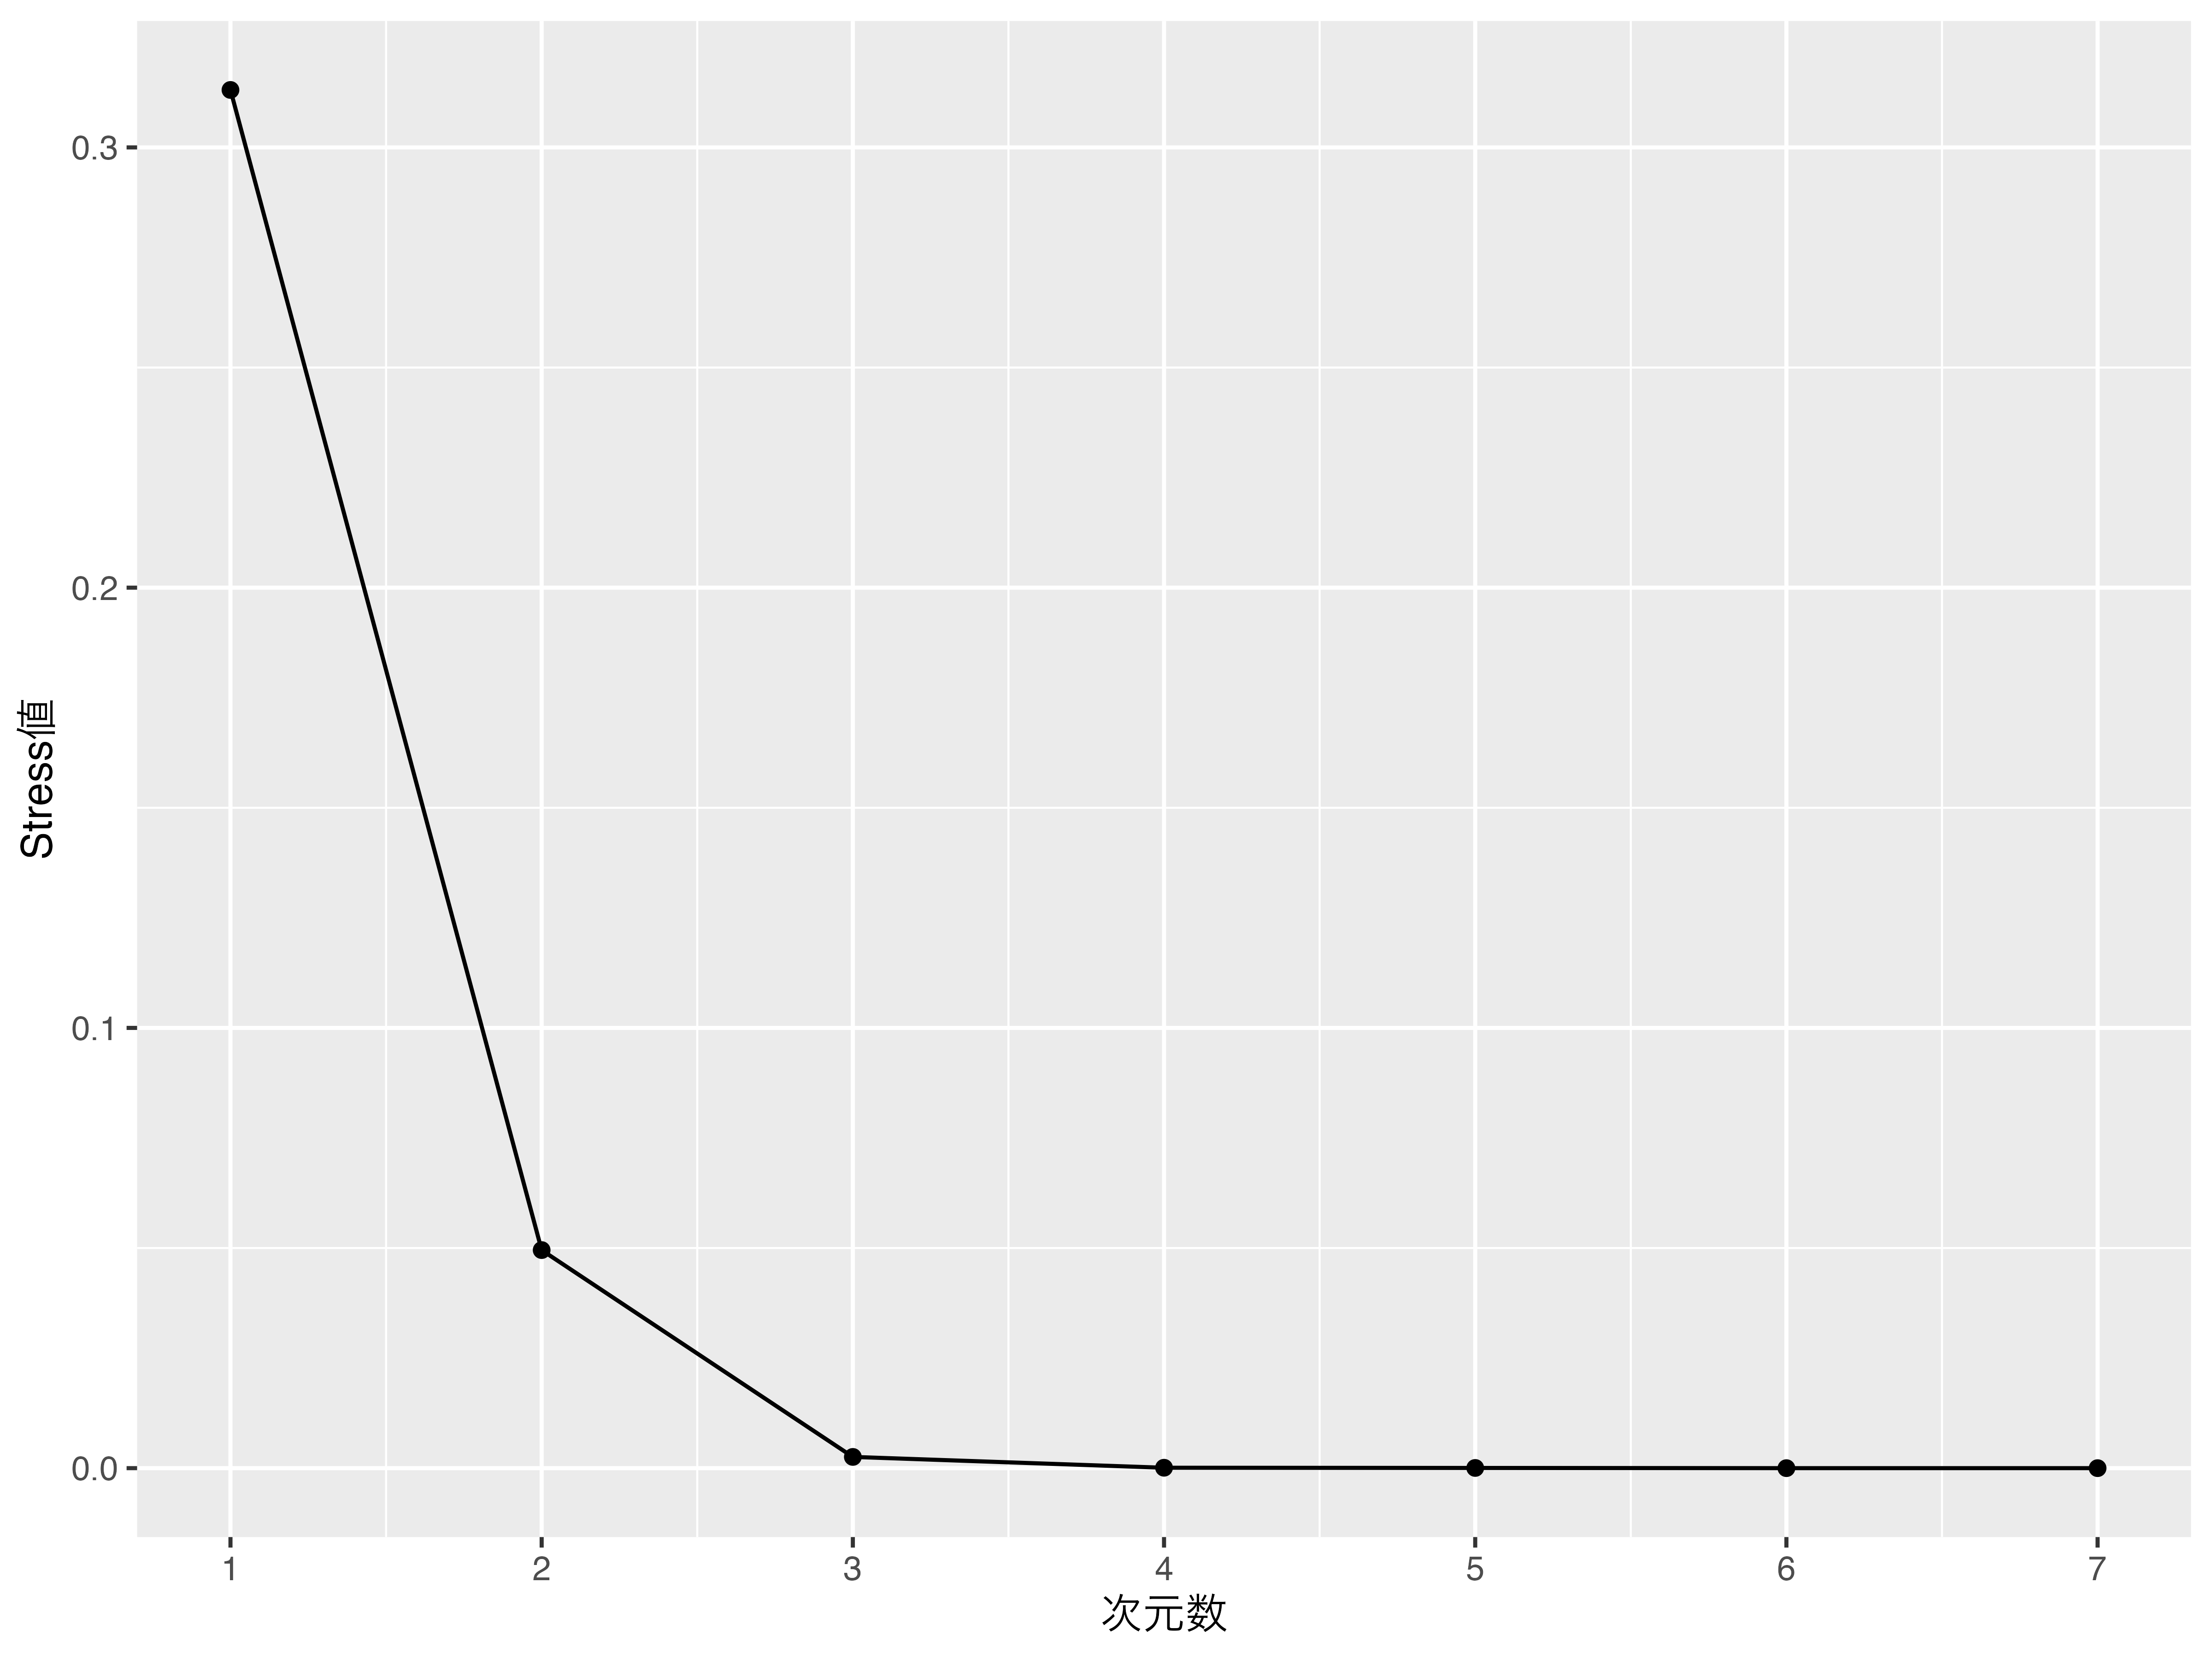
\includegraphics[width=0.8\linewidth,keepaspectratio]{../images/15_MDS/Rplot15_02.png}
		\caption{Stress値の減衰}
		\label{fig::15_02}
	\end{center}
\end{figure}

まるで因子分析の\keytermL{スクリープロット}{すくりーぷろっと}のようですね。横軸に次元数，縦軸にStress値を置いた折れ線グラフですが，当然のことながら反映させるMDS空間の次元数が増えるとデータとの距離が縮んでいきます。
\textcite{kruskal1964multidimensional}の基準によれば，Stress値は表\ref{tbl:x15_stress}のように評価できます。この基準でいくと，今回は2次元で4.9\%(0.0049534)ですから，2次元解でOKとしましょう。

\begin{table}[ht]
	\centering
	\caption{Stress値の評価}
	\begin{tabular}{cc}
		Stress           & Goodness of Fit \\\hline
		20\%             & poor            \\
		10\%             & fair            \\
		5\%              & good            \\
		$2\frac{1}{2}$\% & excellent       \\
		0\%              & ``perfect''     \\\hline
	\end{tabular}
	\label{tbl:x15_stress}
\end{table}

演者をプロットしたのが図\ref{fig::15_03}です。東西南北というか，上下左右の軸に特に意味はありませんから，因子分析のように因子軸の解釈や命名をすることはありません。近くにプロットされた対象は評価が似ていたんだな，ということがわかりますし，相対的な位置関係から，「ハライチとももは芸風が真逆だな」とか「ロングコートダディは中心に近いから中庸的な笑い，悪く言えばキャラが立ってないんだな」といったことが読み取れます。
\begin{figure}[ht]
	\begin{center}
		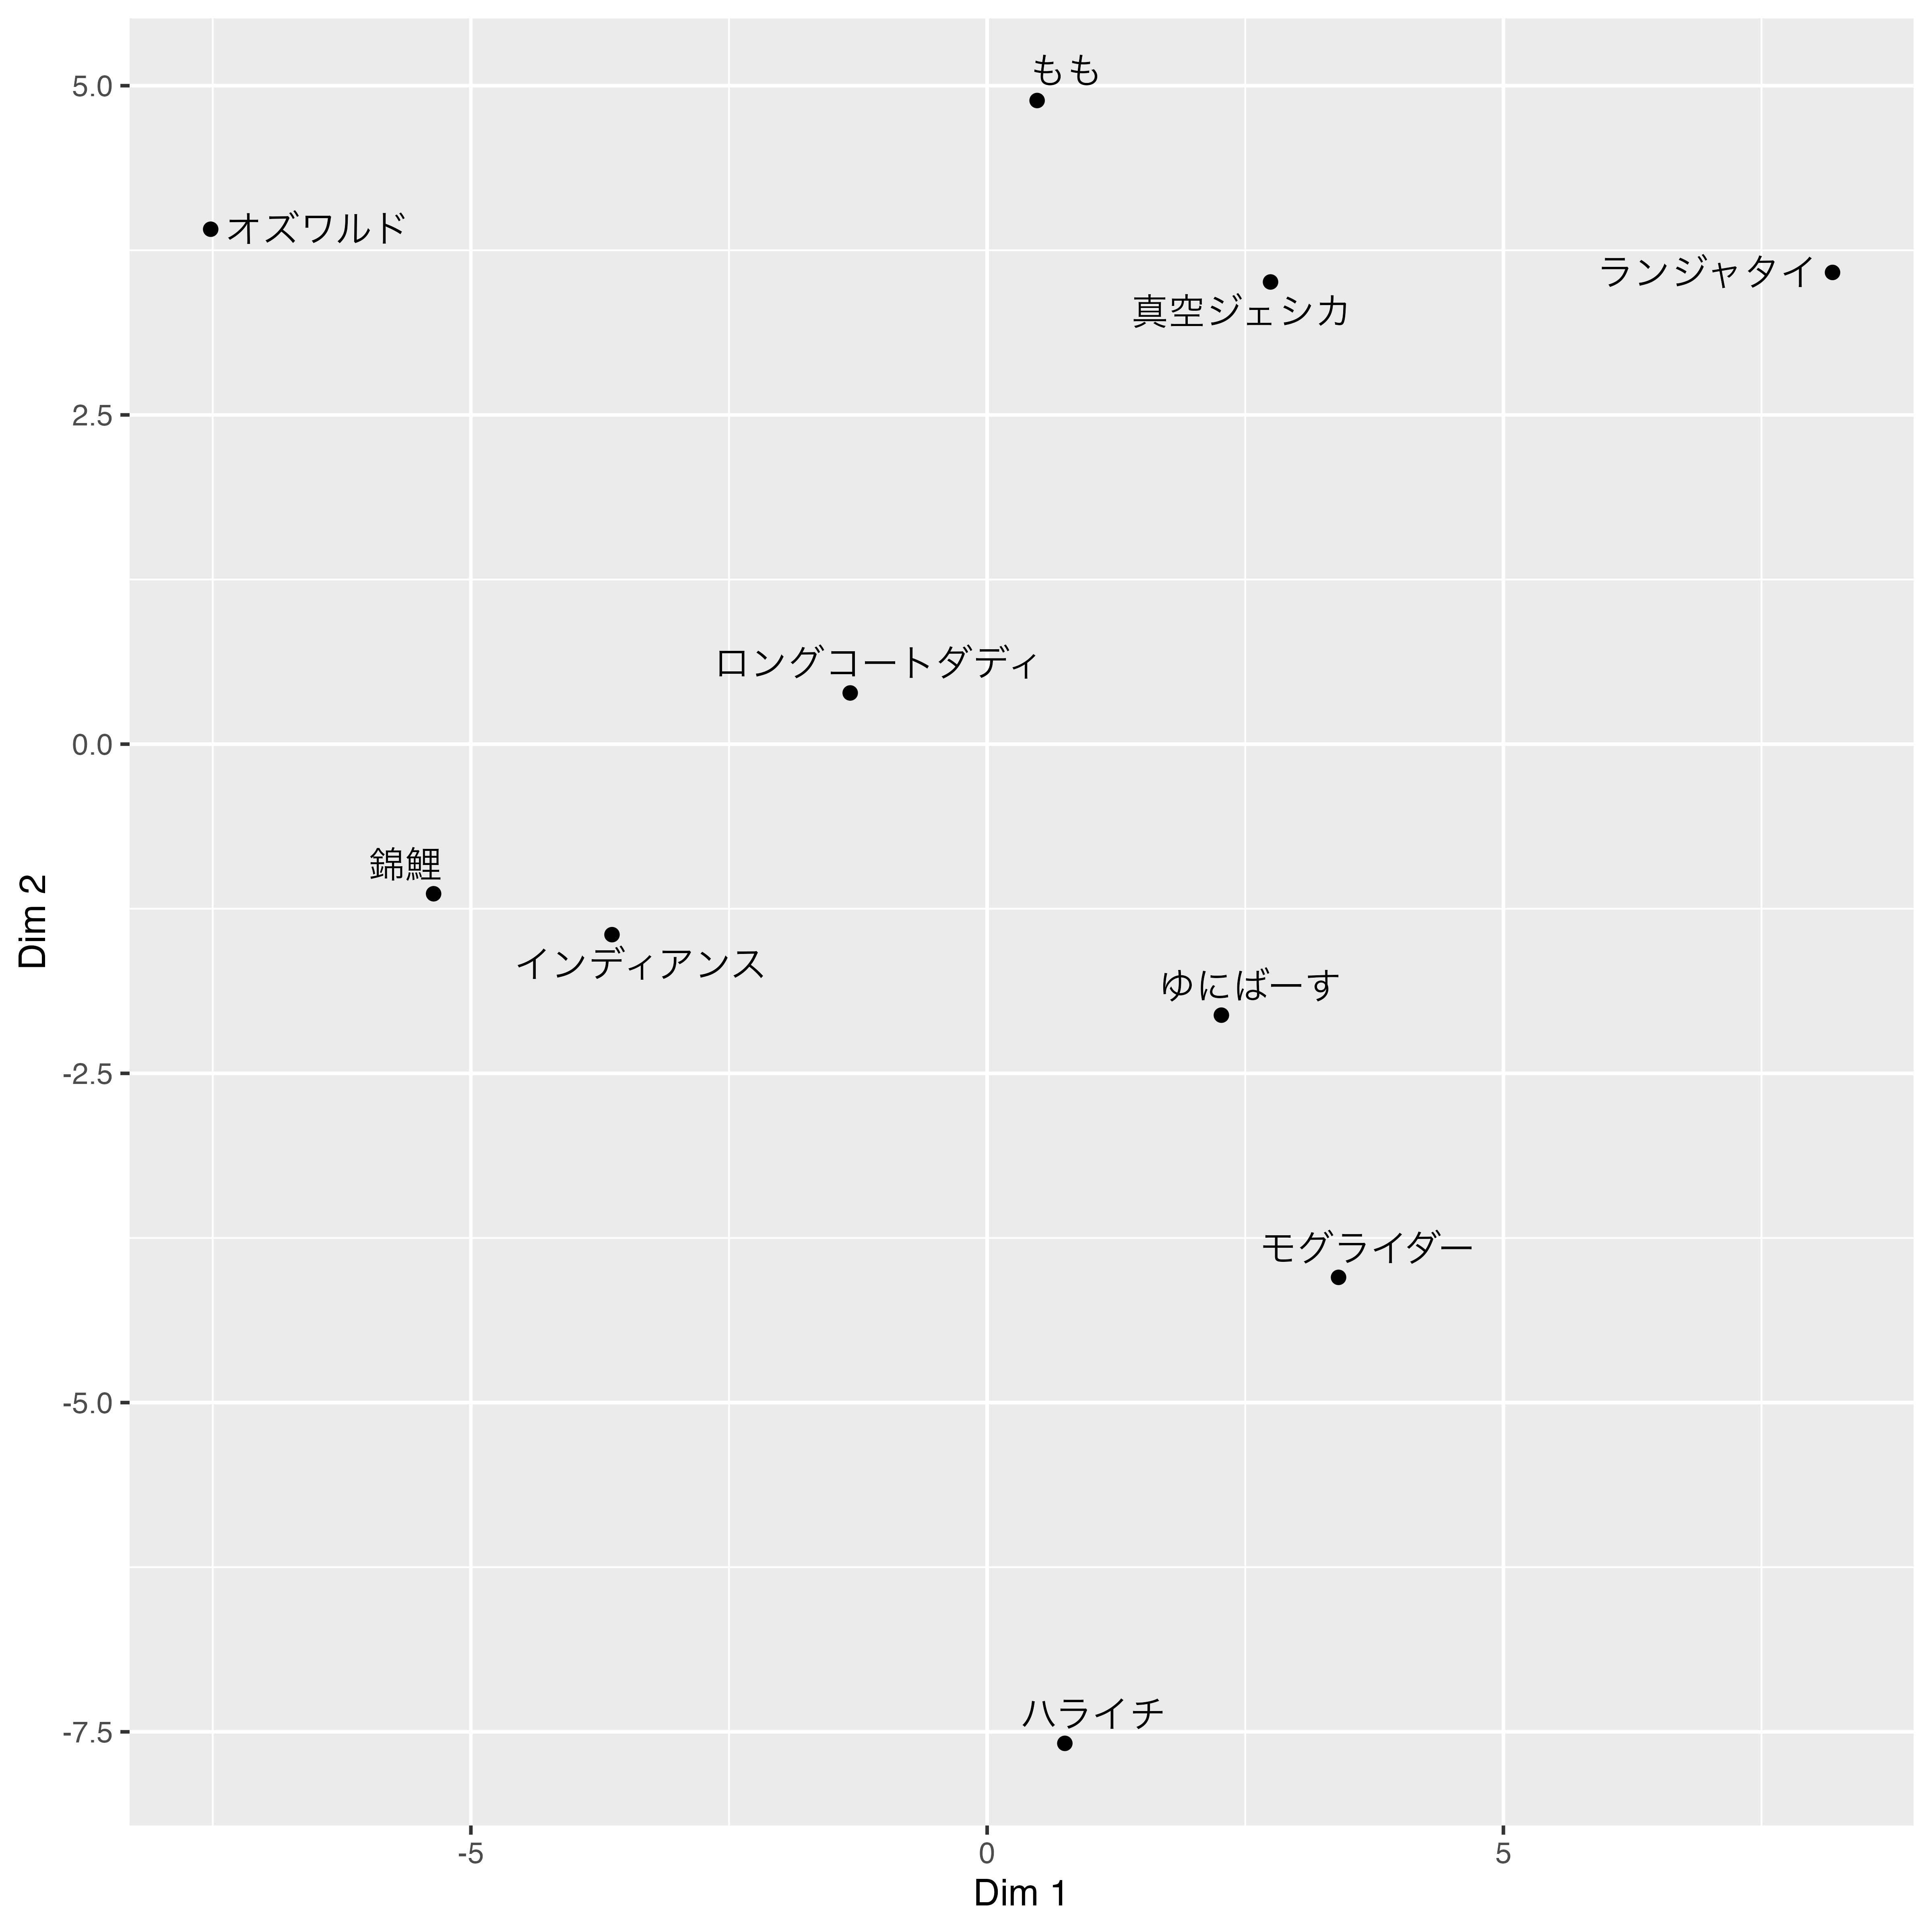
\includegraphics[width=0.8\linewidth,keepaspectratio]{../images/15_MDS/Rplot15_03.png}
		\caption{非計量MDSのプロット}
		\label{fig::15_03}
	\end{center}
\end{figure}
この図\ref{fig::15_01}や図\ref{fig::15_03}のようにMDSで作られた座標のことを特に\keyterm{布置}{ふち}{configure}といいます。特に非計量MDSは優劣・大小関係という順序尺度水準の評定だけからでも，その空間的な特徴を描くことができますから，心理尺度のもつ仮定や測定モデルを考える必要がないため，今後その重要性が再発見されていくのではないかと思います。

\section{多次元尺度法の展開}
多次元尺度構成法で作られた地図は，対象をプロットした地図です。
地図には，その上に何か書き込んだり，地形の図に天気図を重ねるように複数の地図を重ねて表現したりできます。
多次元尺度構成法にも，このような応用モデルがいろいろ考えられています。ここでいくつかの発展的なMDSモデルを見てみましょう。

\paragraph{prefmap}類似度空間の上に，個々人の理想点を追加する方法です。個人の好みpreferenceをマッピングする方法なので，\keyterm{Preference Mapping}{Preference Mapping}{}と呼ばれています。個人$i$が対象$j$について，好みの程度を$s_{ij}$と評価したとします。対象$1,2,...j...,M$は別途類似度評定によって，MDSのつくった地図上にプロットされているとします。ここで個人$i$と対象$j$との地図上の距離$d_{ij}^2$に対して，次の回帰式を考えます。
\[ s_{ij} = a_i d_{ij}^2 + b_i + e_{ij} \]
% つまり，個人$i$と対象$j$の距離を使って，好みの程度$s_{ij}$を予測するモデルを作り，誤差がもっとも小さくなる点に個人$i$をプロットするのです。こうすることで，対象とそれを評価する人を一枚の地図に表現すると言うことができます。
In other words, we create a model to predict the degree of preference $s_{ij}$ using the distance between individual $i$ and object $j$, and plot individual $i$ at the point where the error is smallest. By doing so, we can express the object and the person evaluating it on a single map.

% 例えば先ほどのM-1の例ですが，私の採点では表\ref{tbl:x15_kosugiRatio}のようになりました\footnote{ランジャタイは何が面白いのかわからなかった。モグライダーはもっと評価されるべき。ハライチも良かったですね，ちょっと時間オーバーしたっぽいけど。}。
For example, in the case of the previous M-1, my score was as shown in Table \ref{tbl:x15_kosugiRatio}\footnote{I didn't understand what was interesting about Rangatai. Mograider should be more highly valued. Haraitchi was also good, seemed like it went a bit over time though.}.
\begin{table}[ht]
	\centering
	\caption{著者の評定}
	\begin{tabular}{cc}
		演者        & 採点 \\\hline
		モグライダー    & 90 \\
		ランジャタイ    & 60 \\
		ゆにばーす     & 85 \\
		ハライチ      & 92 \\
		真空ジェシカ    & 83 \\
		オズワルド     & 89 \\
		ロングコートダディ & 85 \\
		錦鯉        & 83 \\
		インディアンス   & 82 \\
		もも        & 88 \\\hline
	\end{tabular}
	\label{tbl:x15_kosugiRatio}
\end{table}

% この評定値を使って著者の理想点を書き足したのが図\ref{fig::15_04}です。低く評価したランジャタイからは遠く，高く評価したハライチやオズワルドに近いところに著者の理想的な笑いの点があり，錦鯉やインディアンスも近くにありますから，今回の優勝にはまぁ納得，と言ったことがわかります。皆さんも自分の理想の点を書き加えてみませんか?
The figure \ref{fig::15_04} is augmented with the author's ideal point using this evaluation value. The author's ideal comedy point is located at a distance from the low-rated Rangatai and close to the highly-rated Haraiti and Oswald. The Koi Carp and Indians are also nearby, so we can understand that we are reasonably convinced with this victory. Why don't you all try adding your own ideal points?
\begin{figure}[ht]
	\begin{center}
		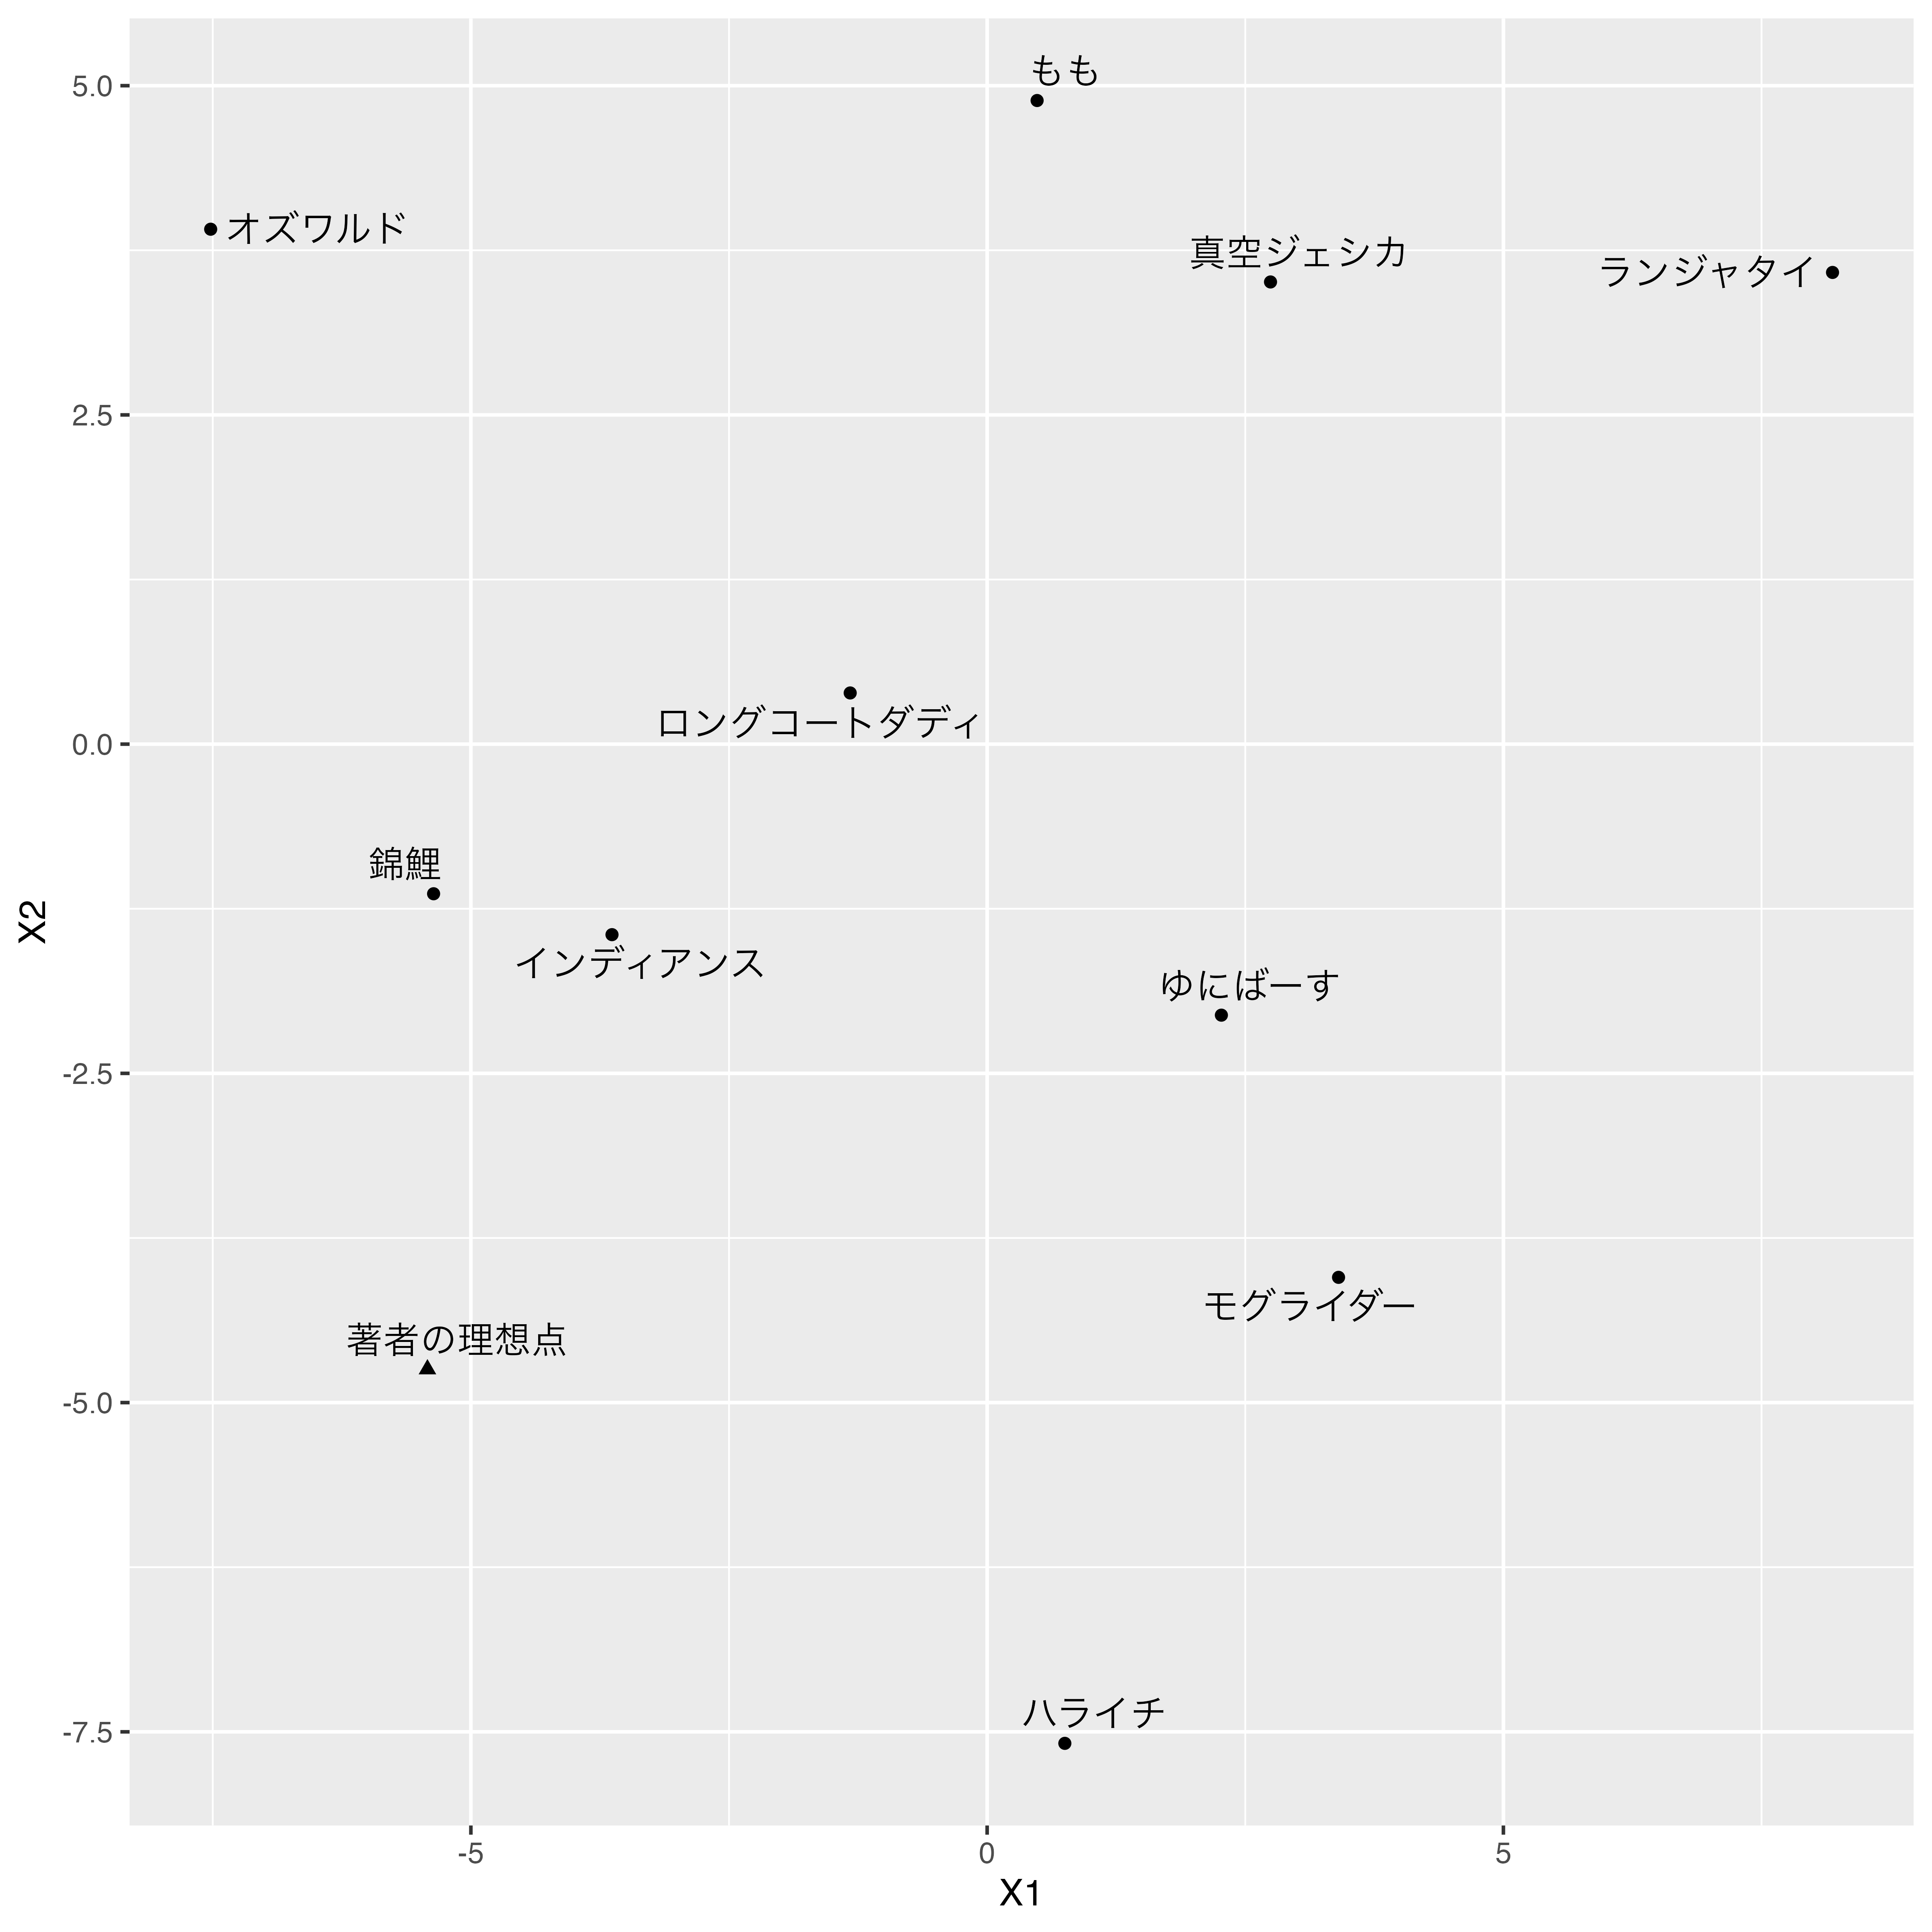
\includegraphics[width=0.8\linewidth,keepaspectratio]{../images/15_MDS/Rplot15_04.png}
		\caption{著者の理想点プロット}
		\label{fig::15_04}
	\end{center}
\end{figure}

% \paragraph{Abelson Map}これは\parencite{abelson1954technique}の考えた手法で，これもprefmapと同じく布置される対象に別の力(選好度でもなんでもよい)があると考え，地図空間上に力の場をプロットして等高線を引くことで表現するモデルです。
\paragraph{Abelson Map} This is a technique devised by \parencite {abelson1954technique}, and like prefmap, it assumes that the object being arranged has another force (preference or anything is ok), and plots the force field on the map space, drawing contour lines to express the model.

% この方法では，各点Pにかかる力$V(P)$を次のように定式化します。
In this method, we formulate the force $V(P)$ acting on each point P as follows.
\[ V(p) = \sum_{j=1}^M \frac{V(j)}{1+d_{pj}^2} \]
ここで$j$は各点，ここで言えば漫才師のことで，$V(j)$が漫才師$j$に与えられた評価点です。$d_{pj}^2$は任意の点$p$と対象$j$の距離ですから，任意の点$p$にかかる力は各漫才師が発する笑い力ですね。

この方法で，先ほどのM-1プロットに，著者の評価をAbelson Mapの方法で描き加えてみましょう。
\begin{figure}[ht]
	\begin{center}
		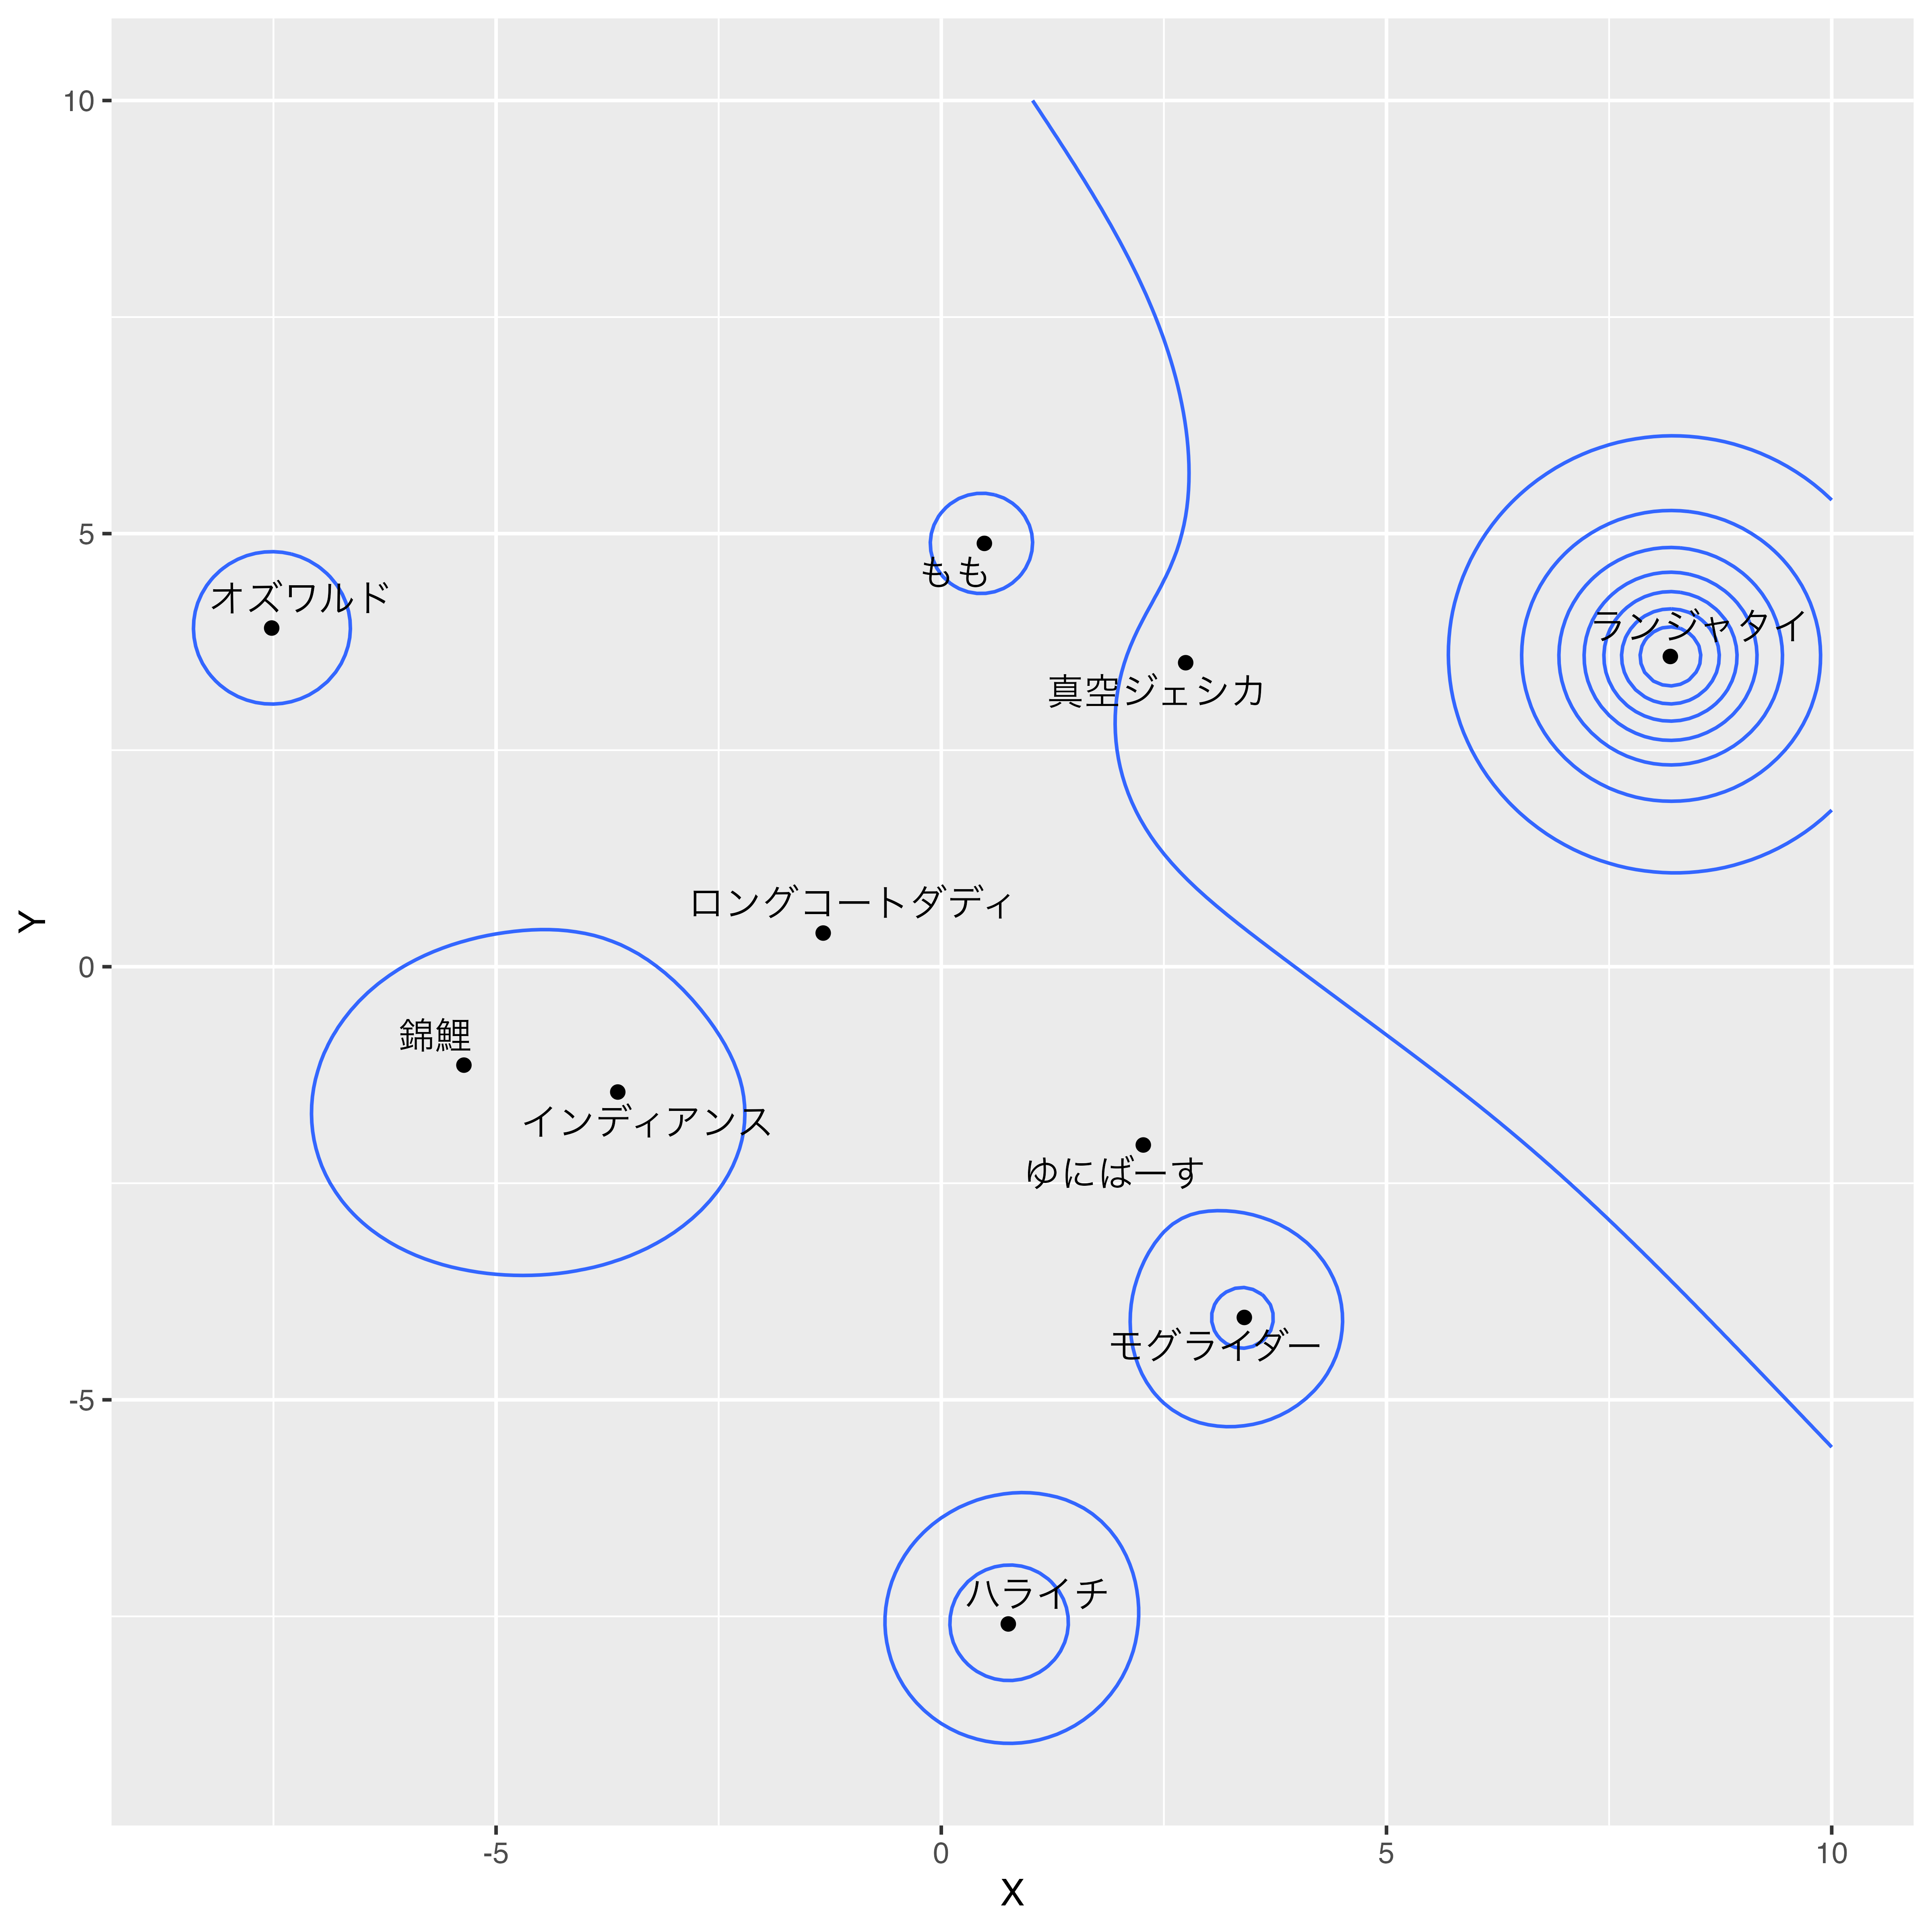
\includegraphics[width=0.8\linewidth,keepaspectratio]{../images/15_MDS/Rplot15_05.png}
		\caption{Abelson Mappingによるお笑い力の等高線図}
		\label{fig::15_05}
	\end{center}
\end{figure}
図\ref{fig::15_05}の右にある，ランジャタイの周りにたくさんの線が引かれていますが，いわばこれは低気圧のようにここのパワーが弱い(と著者は思っている)ところになります。実は，真空ジェシカの左側に通っているラインが平均点のラインですから，ここを境に著者は「面白い」と「面白くない」を区分しているとも言えます。ハライチやオズワルドの周りにある等高線は山の高さ，パワーの強さを表しているラインですね。

力のメタファーにすぎないと言われたらそうですが，このように色々なものを可視化できるのもMDSの面白いところです。

\paragraph{非対称多次元尺度構成法}距離データは対称でなければならない，というものの，たとえば好きな人に振り向いてもらえない＝片想いとか，都市間の人口の流入・流出，国際貿易の赤字・黒字などを考えると，対称間の関係が対称出ないことは少なくないわけです。そうした非対称な関係を，図に加えようと言うのが非対称MDSです。非対称情報を対象部分+歪対象部分に分割し，この対称でない要素を図の中に書き加えるモデルが一般的で，プロットする対象の周りに縁や楕円で表現するとか，矢印で表現するとか，vonMises分布と呼ばれる\keytermL{確率分布}{かくりつぶんぷ}で表現するとか，さきほどのAbelson Mapで高さとして表現するなどのモデルがあります。より数学的なモデルとして，プロットする空間を複素空間にするモデルもあります。詳しくは\textcite{Chino2012}を参考にしてください。

\paragraph{多次元展開法}リッカート法は心理尺度でもっともよく使われる方法で，「非常に当てはまる」から「まったく当てはまらない」までの段階的な反応を被験者に求める方法です。これは\keytermL{段階反応モデル}{だんかいはんのうもでる}で分析されることからも明らかなように，項目に対する反応段階が順番的に強くなっていくことを仮定しています。しかし，実際に被験者が丸をつけるときは，「自分の感覚にもっとも近いカテゴリーを選ぶ」ということをしているはずです。つまり，被験者と反応カテゴリーの距離が，尺度に反映されているはずなのです。この考え方から，尺度に対する反応を距離とし，項目とそれに回答した被験者の両方をプロットする地図を書く方法があります。Coombsが考えた\keyterm{多次元展開法}{たじげんてんかいほう}{Multi-dimensional unfolding method}と呼ばれる手法がそれで，この手法から態度測定の尺度化を考えることもできます。発想としては数量化理論に近く，また\textcite{shimizu2018}はこれを確率モデルに展開しています。

ここであげたいくつかの例にあるように，多次元尺度法もさまざまな角度から人の判断や反応から，\keyterm{尺度}{しゃくど}{scale}を作る方法です。多次元尺度構成法は因子分析モデルよりも制約や仮定が少なく，より直接的に心理的反応をモデル化しようとしています。

本講で学んだように，心理学ではさまざまな角度から「数値化するルール」を考えてきていますが，それぞれ仮定や目的，何を良い尺度と考えるかという観点がことなります。我々心理学者は，統計的なツールのユーザに過ぎません。データは分析できればそれでいい，分析は機械がやってくれるから深く考えなくていい，という割り切り方もあるかもしれませんが，「そもそも何をデータとするか」「どのように数値化するか」という点については，そのような態度は取れないはずです。なぜならそもそも「心はいかにして数値化できるか」ということが明らかでないならば，その後の分析はすべて嘘っぽい数字を使った統計ごっこに過ぎないからです。\textbf{心理学者であるために，われわれは何をどのように数値化しているかについて，しっかりと理解する必要があるのです。}

\section{課題}
計量MDS，非計量MDSをそれぞれ一例ずつ，実践してみてください。データはどのようなものでも構いません。提出ファイル形式はRスクリプトかRmdとします。なお提出されたコード単体でバグがなく動くことが確認できないものは，未提出扱いになります。コードの書き方などわからないところがあれば，曜日別TAか小杉までメールで連絡し，指導を受けてください。


\end{document}
